\section{Cuarto \textit{sprint} de producción}
Una vez definidas las nuevas estrategias de trabajo y que se atendieron
las observaciones de los sinodales se procedió a realizar la maquetación de los
niveles pares restantes y los \textit{sprites} faltantes. Al término de este
\textit{sprint} se obtienen más de 100 \textit{sprites} y las maquetas de los
niveles pares.

\subsection{Creación de las maquetas de los niveles pares restantes}
Para la generación de las maquetas se sigue usando la plantilla creada durante
la creación del primer demo del juego (ver figura \ref{fig:MaquetaPlantilla}).
Para la creación de la maqueta también se crea un documento con todos los
componentes de un nivel como son los enemigos, los ítems, los puntos de guardado,
las plataformas y los obstáculos. Este documento se imprime y los objetos se
recortan para ser pegados como estampas en las plantillas de diseño de las
maquetas. En promedio la maqueta de cada nivel no excede de las 15 plantillas,
sin embargo hay algunas que exceden este número como la maqueta del cuarto nivel,
la cual por su naturaleza de laberinto terminó por ser más extensa que el
resto. Por su parte los niveles correspondientes a los jefes de los niveles no
sobrepasan de las tres plantillas, siendo la maqueta del jefe del sexto nivel
la más pequeña de todas.

%%
\begin{figure}[h]
    \centering
    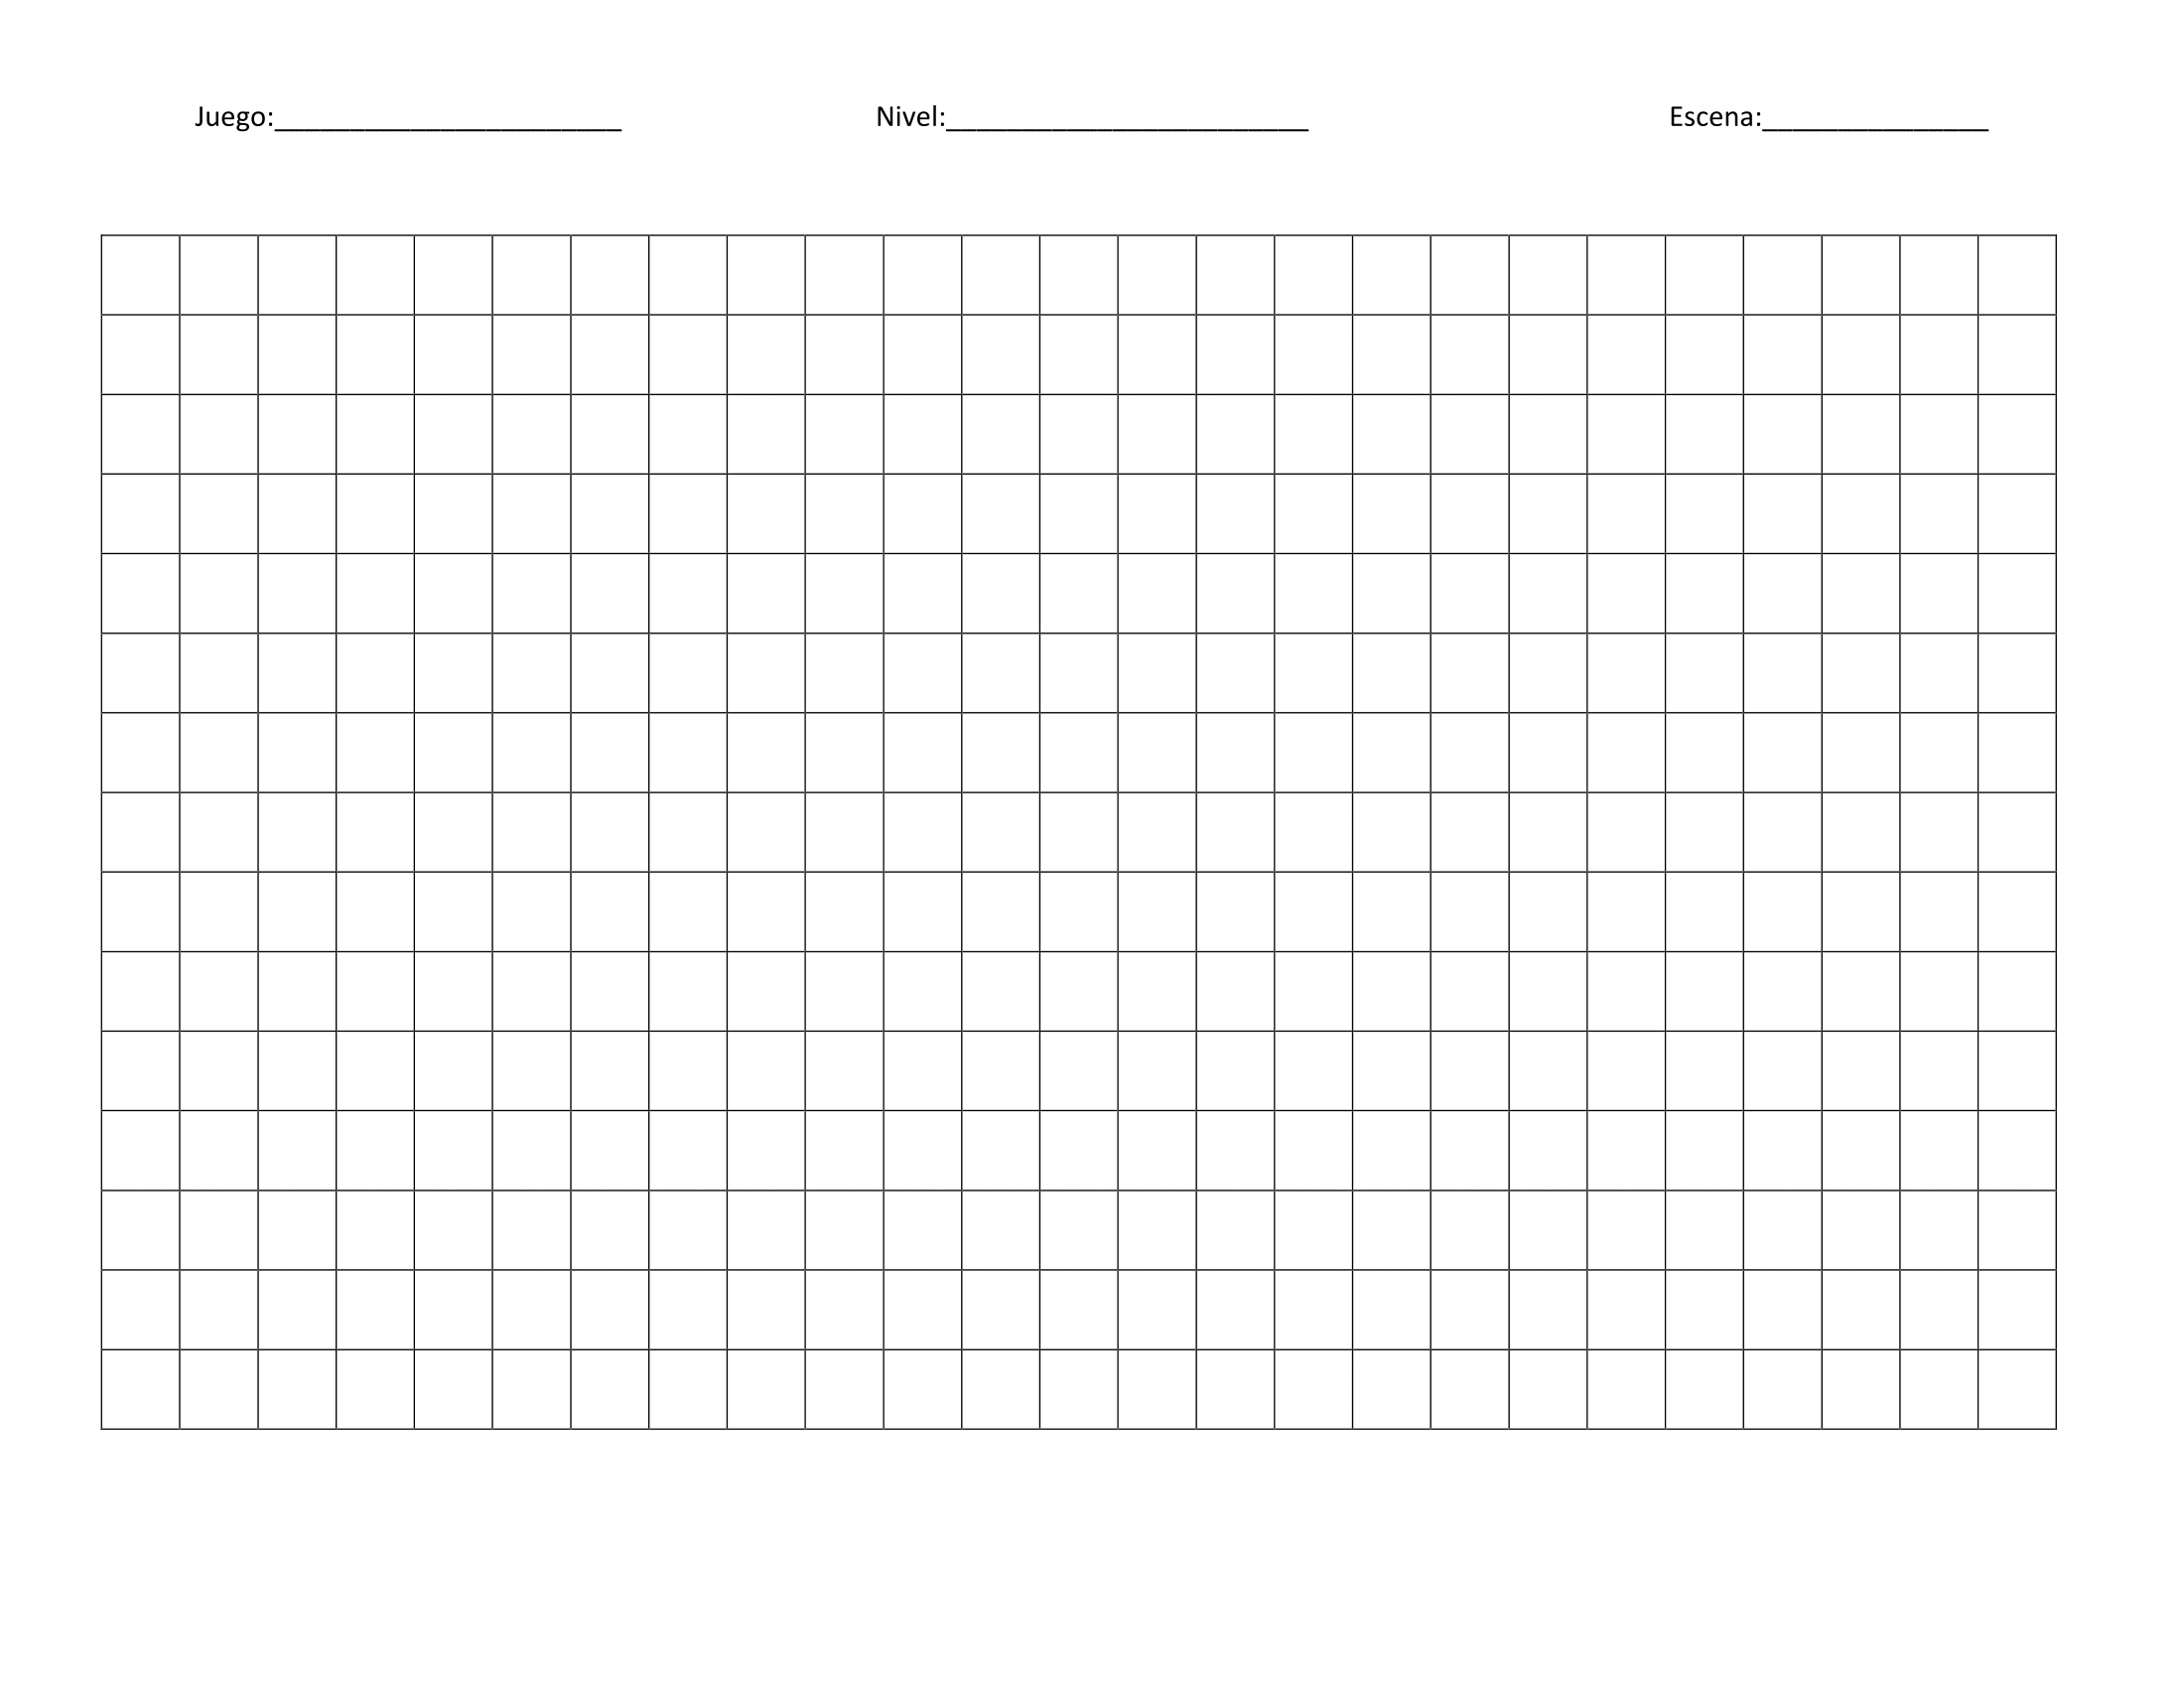
\includegraphics[width=0.6\textwidth]{03TrabajoRealizado/imagenes/maqueta-1.png}
     \caption{Plantilla para la creación de niveles.}
    \label{fig:MaquetaPlantilla}        
\end{figure}

\subsection{Creación de los \textit{sprites} faltantes}
Lo siguiente a realizarse durante el cuarto \textit{sprint} fueron los \textit{sprites},
durante las modificaciones que se definieron en Trabajo Terminal 1 fue la
utilización de un \textit{software} de animación en dos dimensiones para generar
los \textit{sprites} restantes; sin embargo, el cambio de \textit{software} para
generar los sprites fue descartado, esto debido a que se adquirió una nueva
tableta digitalizadora que agiliza la creación de \textit{sprites}. Para Trabajo
Terminal 2 se dibujaron y digitalizaron más de 100 \textit{sprites}. Para mejorar
la experiencia visual del jugador se animaron \textit{sprites} que en los primeros
demos eran estáticos como es el caso de los fantasmas del segundo nivel de la
sección de plataformas (ver figura \ref{fig:FantasmaAnimacion}).

%%
\begin{figure}[h]
    \centering
    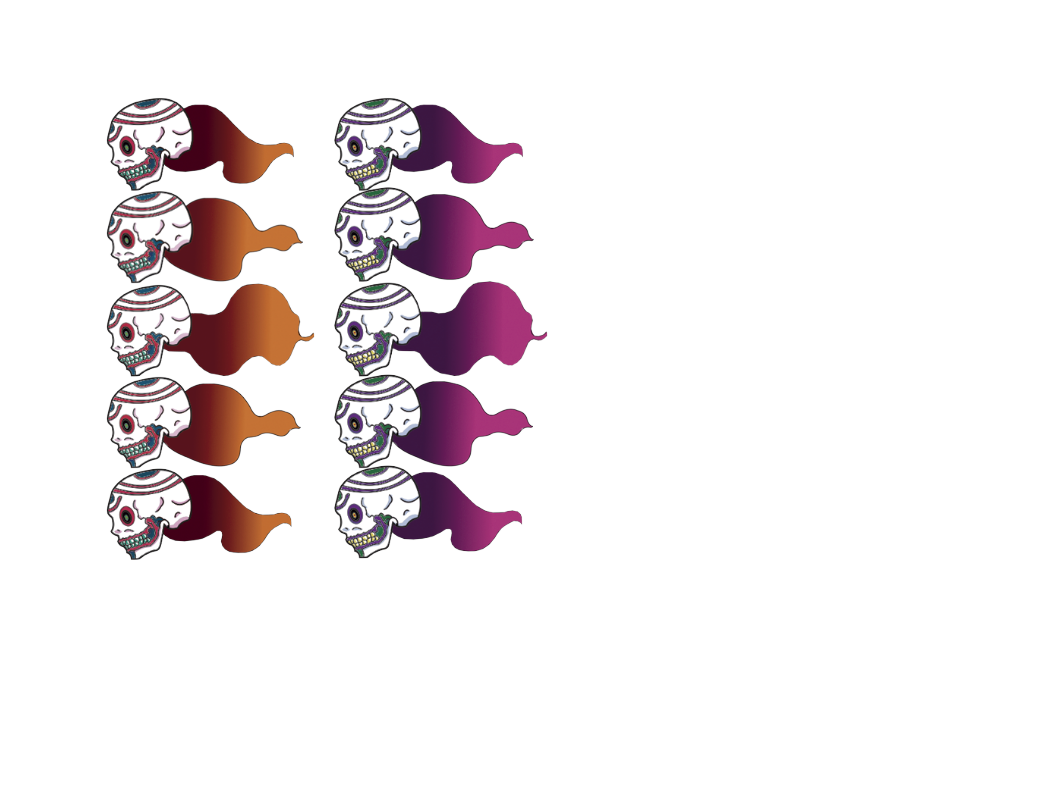
\includegraphics[width=0.6\textwidth]{03TrabajoRealizado/imagenes/fantasmas.png}
     \caption{Bloques de animación para el enemigo de tipo fantasma.}
    \label{fig:FantasmaAnimacion}        
\end{figure}

Otros cambios en cuanto el aspecto visual del juego fue la integración de nuevos
\textit{sprites} para el personaje jugable, los nuevos sprites incluyen la
caracola que \textit{Malinalli} (ver figura \ref{fig:MalinalliCaracola}) emplea
para atacar y que se obtiene al final del primer nivel de la sección de selva,
estos \textit{sprites} para \textit{Malinalli} son utilizados únicamente en los
niveles posteriores al primer nivel para darle sentido a la narrativa; para el
segundo nivel se hizo algo parecido, los \textit{sprites} del personaje jugable
fueron sustituidos por \textit{Malinalli} montando un ajolote (ver figura
\ref{fig:MalinalliAjolote}), este cambio se hizo para que lo que el jugador vea
dentro del nivel sea coherente con la narrativa propuesta y se mejore la inmersión del juego.

\begin{figure}[h]
    \centering
    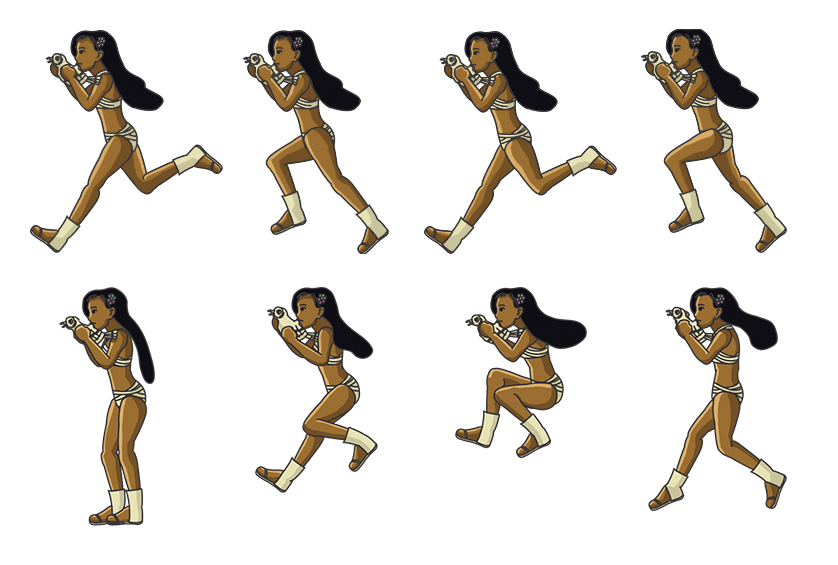
\includegraphics[width=0.4\textwidth]{03TrabajoRealizado/imagenes/MalinalliArma.png}
     \caption{Bloques de animación para \textit{Malinalli} posterior a que ella obtiene la caracola.}
    \label{fig:MalinalliCaracola}        
\end{figure}

\begin{figure}[h]
    \centering
    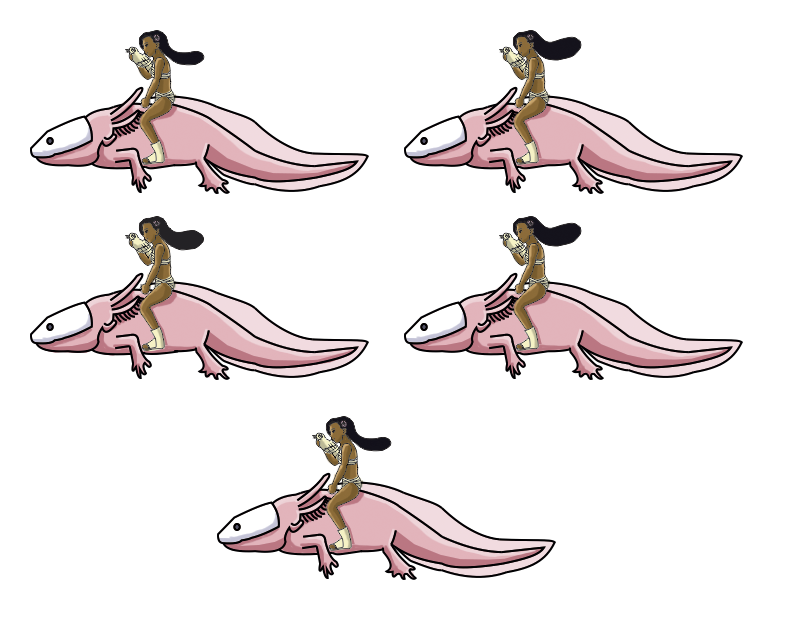
\includegraphics[width=0.5\textwidth]{03TrabajoRealizado/imagenes/MalinaliAjolote.png}
     \caption{Bloques de animación para \textit{Malinalli} montando al ajolote del segundo nivel del juego.}
    \label{fig:MalinalliAjolote}        
\end{figure}

En lo que se refiere a los Jefes de cada nivel, no solo se crearon sus
respectivos \textit{sprites}, también fue necesario la creación de los
\textit{sprites} referentes a sus ataques, para el caso particular de
\textit{Mictlantecuhtli} se dibujaron 30 \textit{sprites} tanto para la animación
del personaje como para la animación de sus respectivos ataque (ver figura
\ref{fig:Mictlantecutli}). Para el diseño de la interfaz gráfica de usuario
(\textit{GUI} por sus siglas en inglés) se emplearon \textit{sprites} de las
paginas \textit{Kenney.nl} y \textit{Game Art 2D}. Es importante aclarar que la
creación de \textit{sprites} pudo haber sido sustituida utilizando paquetes de
\textit{sprites} que existen en la red y que son de licencia libre; sin embargo,
con la creación de \textit{sprites} propios para el juego se consigue crear una
identidad visual propia al juego, esto permite que el jugador se identifique con
mayor facilidad con el personaje y tenga una mejor asociación con el mundo y la
historia que se le presenta dentro del juego [cita]. Si se desea ver a profundidad
los {sprites} que se crearon se puede consultar el anexo \ref{Anexo:Personajes}.

\begin{figure}[h]
    \centering
    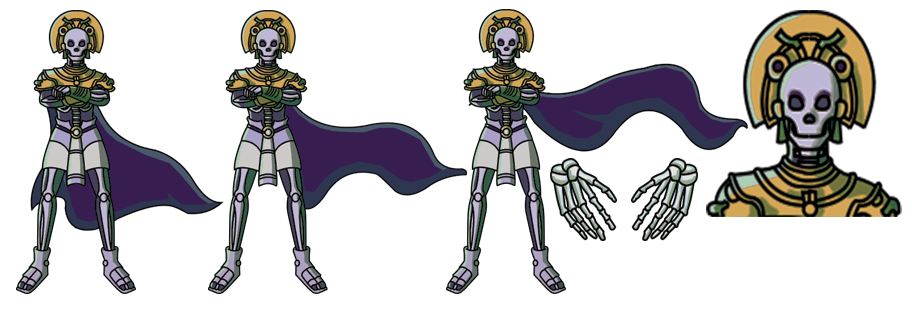
\includegraphics[width=0.6\textwidth]{03TrabajoRealizado/imagenes/Mictlantecuhtli.png}
     \caption{Bloques de animación para \textit{Mictlantecuhtli}, jefe final del juego.}
    \label{fig:Mictlantecutli}        
\end{figure}

\subsection{Cierre del sprint}
Al terminar este \textit{sprint} se obtienen todas las maquetas de los niveles
pares y los \textit{sprites} a utilizar de los mismos. Este \textit{sprint} se
considera completado ya que se generaron todos los elementos que se tenían
planeado. Como último paso para este \textit{sprint}, se realiza el empaquetado
de todos los \textit{sprites} creados durante el \textit{sprint}.

